\section{Current of Electricity}
\subsection{Electric current}
\textbf{Elementary charge}:
\[ e = 1.6 \times 10^{-19}\:\unit{C} \]
\begin{itemize}
\item Protons are positively charged, with a charge $+e$.
\item Electrons are negatively charged, with a charge $-e$. 
\item Ions carry charges that are multiples of $+e$ and $-e$.
\end{itemize}

\begin{defn}{Electric current $I$}{}
Rate of flow of charge.
\[ I=\odv{Q}{t} \]
For a steady current $I$, we have 
\begin{equation}
Q = It
\end{equation}
\end{defn}

\begin{remark}
By convention, the direction of current is the direction that \underline{positive charges} move. However, remember that current is due to the flow of \underline{electrons}; lattice atoms/ions do not move.
\end{remark}

\textbf{Transport equation}:
\begin{equation}
I=nAvq
\end{equation}
where $v$ is the \textbf{drift velocity}.

\begin{figure}[H]
    \centering
    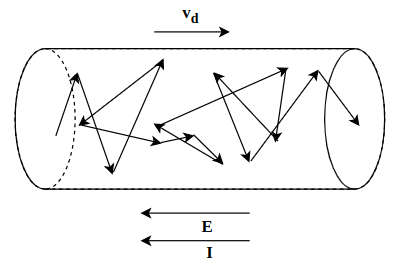
\includegraphics[width=8cm]{images/transport_eqn.png}
\end{figure}

\begin{remark}
Drift velocity of charge carriers is much lower than the maximum velocity that charge carriers could achieve from the potential difference applied to the wire.

This is because charge carriers experience electrical force in \underline{all directions} because of collisions with lattice ions. This produces a range of velocities. The drift velocity is an \underline{average}.
\end{remark}

\begin{remark}
When a domestic lighting circuit is switched on, the lights come on almost immediately. 
This is because when the switch is on, all electrons in the wire and filament start to move \underline{together}.
\end{remark}
\pagebreak

\subsection{Potential difference and electromotive force}
\begin{defn}{Potential difference $V$}{}
\underline{Work done per unit charge} when electrical energy is converted into non-electrical energy when the charge passes \underline{from one point to the other}.
\begin{equation}
V = \frac{W}{Q}
\end{equation}
\end{defn}

\begin{defn}{Electromotive force $\epsilon$}{}
\underline{Work done per unit charge} when non-electrical energy is converted into electrical energy when the charge is moved \underline{around a complete circuit}.
\begin{equation}
\epsilon = \frac{W}{Q}
\end{equation}
\end{defn}

\begin{table}[H]
\centering
\begin{tabular}{|p{7.5cm}|p{7.5cm}|}
\hline
\textbf{Potential difference} & \textbf{Electromotive force} \\
\hline
Refers only to source & Refers to any two points in the circuit \\
Amount of non-electrical energy converted into electrical energy & Amount of electrical energy into non-electrical energy \\
Always exists as it is a source of energy & Only exists if current is flowing \\
\hline
\end{tabular}
\end{table}

\begin{figure}[H]
    \centering
    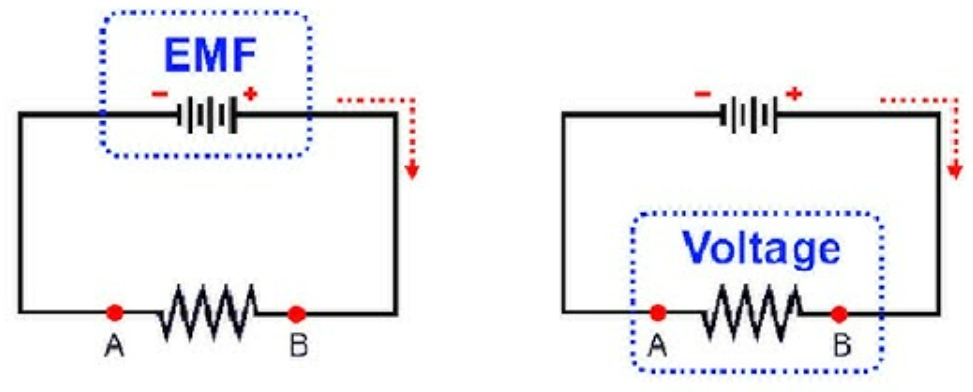
\includegraphics[width=10cm]{images/pd_emf.png}
\end{figure}
\pagebreak

\subsection{Resistance}
\begin{defn}{Resistance $R$}{}
\underline{Ratio} of potential difference across component to current flowing through it.
\begin{equation}
R = \frac{V}{I}
\end{equation}
\end{defn}

\textbf{Resistivity} is a property unique to the material.
\begin{equation}
R = \rho \frac{l}{A}
\end{equation}

\begin{defn}{Ohm's Law}{}
Current flowing through conductor is directly proportional to potential difference applied across it, provided that \underline{physical conditions remain constant}.
\begin{equation}
I \propto V
\end{equation}
\end{defn}
\pagebreak

\subsection{I-V characteristics}
An ohmic resistor obeys Ohm's Law. For non-ohmic resistors that do not obey Ohm's Law, factors that cause resistance to deviate are:
\begin{enumerate}
\item Number density of charge carriers $n$ (decrease resistance)
\item Amplitude of atomic vibrations of lattice atoms (increase resistance)
\end{enumerate}

\subsubsection{Ohmic resistor}

\begin{figure}[H]
\centering
\begin{tikzpicture}
  \begin{axis}%
    [axis lines=middle,
     enlargelimits={abs=0.2},
     xlabel = $V$,
     ylabel = $I$,
     ticks=none
    ]
    \addplot[domain=-2:2,samples=50,smooth,red] {x};
  \end{axis}
\end{tikzpicture}
\end{figure}

Resistance is \textbf{constant}: as p.d. increases, current increases proportionately.

\subsubsection{Filament lamp}

\begin{figure}[H]
\centering
\begin{tikzpicture}
  \begin{axis}%
    [axis lines=middle,
     enlargelimits={abs=0.2},
     xlabel = $V$,
     ylabel = $I$,
     ticks=none
    ]
    \addplot[domain=-1.57:1.57,samples=50,smooth,red] {sin(deg(x))};
  \end{axis}
\end{tikzpicture}
\end{figure}

Resistance \textbf{increases}: as p.d. increases, current increases less than proportionately.

\begin{tcolorbox}
\textbf{Alternative explanation:}

The gradient of the line joining the origin to each point on the curve decreases as p.d. increases.

Since resistance is the reciprocal of the gradient, resistance increases as p.d. increases.
\end{tcolorbox}

\begin{itemize}
\item \underline{As temperature increases}, amplitude of atomic vibrations of lattice atoms increases.
\item $n$ does not increase significantly. 
\item Overall effect is resistance increases.
\end{itemize}

\textbf{Useful problem solving technique:}

To find a particular resistance value on an $I-V$ graph, draw the $I-V$ graph of an ohmic conductor with the particular resistance value.

\subsubsection{Semiconductor diode}

\begin{tcolorbox}
\textbf{What is a semiconductor diode?}

A diode is a two-terminal electronic component that has a \underline{low resistance} to the flow of current in one direction thus allowing the passage of current in one direction (\textbf{forward bias}) whereas there will be a \underline{high resistance} in the other, thus restricting the flow of current in that direction (\textbf{reverse bias}).
\end{tcolorbox}

\begin{figure}[H]
\centering
\begin{tikzpicture}
  \begin{axis}%
    [axis lines=middle,
     enlargelimits={abs=0.2},
     xlabel = $V$,
     ylabel = $I$,
     ticks=none
    ]
    \addplot[domain=0:5,samples=50,smooth,red] {x^3};
    \addplot[domain=-2:0,samples=50,smooth,red] {0.0};
    \addplot[domain=-4.5:-2,samples=50,smooth,red] {(x+2)^5};
  \end{axis}
\end{tikzpicture}
\end{figure}

For forward-biased region, resistance \textbf{decreases}: as p.d. increases, current increases more than proportionately.

\begin{itemize}
\item \underline{As temperature increases}, electrons in semiconductor are more likely to have sufficient energy to escape from atom, so $n$ increases significantly.
\item Increase in rate of interaction of electrons with vibrating atoms.
\item Increase in $n$ \underline{predominates over} increase in rate of interactions of electrons with lattice. Overall effect is resistance decreases.
\end{itemize}

For reverse-biased region, resistance is \textbf{infinitely high}: no current flow through diode until breakdown voltage.
\pagebreak

\subsubsection{Negative Temperature Coefficient (NTC) thermistor}

\begin{figure}[H]
\centering
\begin{tikzpicture}
  \begin{axis}%
    [axis lines=middle,
     enlargelimits={abs=0.2},
     xlabel = $V$,
     ylabel = $I$,
     ticks=none
    ]
    \addplot[domain=-2:2,samples=50,smooth,red] {x^3};
  \end{axis}
\end{tikzpicture}
\end{figure}

Resistance \textbf{decreases}: as p.d. increases, current increases more than proportionately.

\begin{itemize}
\item \underline{As temperature increases}, electrons are more likely to have sufficient energy to escape from atom, so $n$ increases significantly.
\item Increase in rate of interaction of electrons with vibrating atoms.
\item Increase in $n$ \underline{predominates over} rate of interactions of electrons with lattice. Overall effect is resistance decreases.
\end{itemize}

\begin{remark}
As temperature of thermistor increases, its resistance decreases.

Since e.m.f. of battery remains unchanged, current increases when resistance decreases, causing greater power to be generated in the thermistor.

This will result in a further increase in temperature of thermistor, decrease in its resistance, leading to \textbf{thermal runaway} which could cause overheating.
\end{remark}

Resistance-temperature characteristic: resistance decreases as temperature increases

\begin{figure}[H]
\centering
\begin{tikzpicture}
  \begin{axis}%
    [axis lines=middle,
     enlargelimits={abs=0.2},
     xlabel = $T$,
     ylabel = $R$,
     ticks=none
    ]
    \addplot[domain=0:5,samples=50,smooth,red] {1/x};
  \end{axis}
\end{tikzpicture}
\end{figure}

\subsubsection{Light Dependent Resistor (LDR)}
Similar to NTC thermistor.
\pagebreak

\subsection{Power}
Electrical power dissipated by the conductor:
\begin{equation}
\begin{split}
P &= VI \\
P &= I^2R \\
P &= \frac{V^2}{R}
\end{split}
\end{equation}

\subsection{Internal resistance}
Let $r$ denote internal resistance of battery, $R$ denote resistance of load, $V$ denote terminal p.d. of battery, $\epsilon$ denote e.m.f.

For an \textbf{ideal} battery, $r=0$. This gives us 
\[ \epsilon=V \]

For a \textbf{real} battery, $r\neq 0$. We imagine the internal resistance as another load of resistance $r$ connected with $R$ in series. 

\begin{figure}[H]
    \centering
    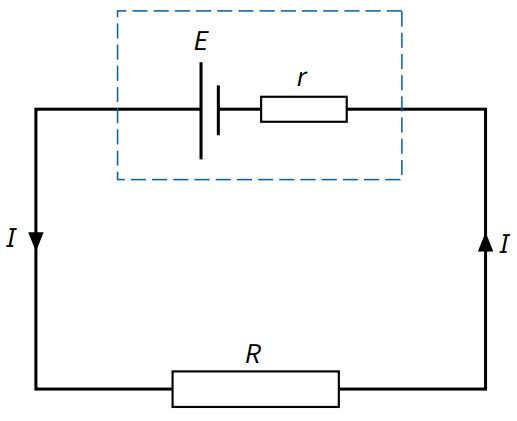
\includegraphics[width=8cm]{images/internal_resistance.jpg}
\end{figure}

Since e.m.f. is sum of p.d., 
\[ \epsilon=I(R+r) \]
\begin{equation}
\epsilon=V+Ir
\end{equation}

This gives us
\[ \boxed{I=\frac{\epsilon}{R+r}} \]

\pagebreak

\subsection*{Problems}
\begin{prbm}
The terminals of a battery are connected to a load resistance. As the battery increases, its internal resistance increases. How does this affect the ability of the battery to deliver energy?
\end{prbm}

\begin{proof}[Answer]
Terminal p.d. decreases. Power delivered to the load decreases (p.d. decrease, resistance constant) as more energy dissipated as heat by internal resistance of battery.
\end{proof}

\begin{prbm}
By considering a practical source with e.m.f. $E$ and internal resistance $r$ connected in series with an electrical device of resistance $R$, determine
\begin{enumerate}[label=(\roman*)]
\item an expression for output efficiency of the source, $\eta=\dfrac{\text{useful power output}}{\text{total power generated}}$.
\item the value of $R$ in terms of $r$ such that maximum power is delivered to the device, and the output efficiency of the source when it is used to operate an electrical device at maximum power.
\end{enumerate}
\end{prbm}

\begin{proof}[Answer] \
\begin{enumerate}[label=(\roman*)]
\item Total power generated:
\[ P_{gen}=I^2(R+r) \]

Useful power output:
\[ P_{out}=I^2R \]

Efficiency:
\[ \boxed{\eta = \frac{R}{R+r}} \]

\item Current in the circuit:
\[ I = \frac{E}{R+r} \]

Power output at the load:
\[ P_{out} = I^2R = \brac{\frac{E}{R+r}}^2R \]

For maximum power output,
\[ \dv{P_{out}}{R} = 0 \implies \boxed{R=r} \]

Output efficiency is \boxed{0.5} (50\%).
\end{enumerate}
\end{proof}
\pagebreak